\chapter{Appendix}
\section{Signals Trajectory Generation}\label{sec:app.casec}
Figure \ref{fig:set.caseA}, \ref{fig:set.xLdB} and \ref{fig:set.xLdC} show the trajectories that are generated for Cases A, B and C. 
This section gives more detail on the generation of the signals that were used in the generation of the trajectories, see Figure \ref{fig:app.casec}.\\
Signal A is the x-component in Case C, and is composed by taking $ \pi \, rad $ of a sine wave with frequency $ \omega=2\pi/45 \frac{rad}{s} $, from the lowest to the highest point. Biasing the signal will make it start smoothly from $ 0 $. This signal is kept constant at $ 20 s $ and multiplied with a gain of $ 20 $. \\
Signal B and signal C are both sine waves with $ \omega=\frac2\pi/3\frac{rad}{s} $ and $ \omega=2\pi/1.5\frac{rad}{s} $. \\
%Signal B  where signal C is used for.
Signal D is a concatenation of a smooth upwards signal, a constant and a smooth downwards signal. The up- and downwards signal are part of a sine wave with frequency $ \omega=2\pi/45\frac{rad}{s} $, composed the same way as signal A.
Signal D is multiplied with signal B and C to ensure that the trajectory gradually increases and decreases.
The multiplication with signal B gives the y-component in case B and case C, and the multiplication with signal C gives the z-component of case C.
%the y- and z-component, ensuring  see Figure \ref{fig:app.casec}, signal D.

%\begin{figure}[h!]
%	\centering
%	\makebox[.49\textwidth][c]{\subfloat[][\label{fig:app.xLdesC}]{\includegraphics[width=.45\textwidth]{\dir{LPOSQRL-xLdes\caseC}}}}
%	\caption{Desired load Position Case C}
%\end{figure}

\begin{figure}[h!]
	\centering
%	\makebox[.49\textwidth][c]{\subfloat[][]{\includegraphics[width=.45\textwidth]{./StyleStuff/dcsc.png}}}
		\makebox[.49\textwidth][c]{{\includegraphics[width=.45\textwidth]{\dir{LPOSQRL-allcasesig\caseC}}}}
		\caption{Signals for trajectory generation\label{fig:app.casec}}
\end{figure}		

%\begin{table}[h!]
%	\centering
%	\begin{tabular}{|l|l|}
%		\hline
%		\textbf{Signal}&$ \omega [rad/s] $\\
%		\hline
%		A & $$\\
%		B & $ $\\
%		C &$ $ \\
%		\hline
%	\end{tabular}
%	\caption{Caption}
%	\label{tab:set.}
%\end{table}


%\section{Derivation of Equations of motion}
%\subsection{Load Dynamics}\label{sec:app.loaddyn}
%%PROOF prop.3 Sreenath2013a. Also Sreenath2013b?
%%DEFINE e_3 / R / f 
%
%Let \lsymb{$ x_{CM} $}{Position CM of \a{qr}-load system} denote the position of the center of mass of the combined quadrotor-load system, expressed in \IF. Which can be found by
%\begin{align}\label{eq:CM}
%\begin{split}
%m_Q(x_Q-x_{CM})+m_L(x_L-x_{CM})&=0\\
%(m_Q+m_L)x_{CM}&=m_Qx_Q+m_Lx_L
%\end{split}
%\end{align}
%Applying Newton's laws of motion to (\ref{eq:CM}) and inserting (\ref{eq:mod.xQ2xL}) gives the 
%\begin{align}\label{key}
%\begin{split}
%(m_Q+m_L)\ddot{x}_{CM}&=fRe_3 - (m_Q+m_L)ge_3\\
%%&=fRe_3 - (m_Q+m_L)ge_3\\
%%(m_Q+m_L)\ddot{x}_{CM}&=m_Q\ddot{x}_Q + m_L\ddot{x}_L\\
%%\\
%%m_Q\ddot{x}_Q+m_L\ddot{x}_L&=fRe_3 - (m_Q+m_L)ge_3\\
%%m_Q(\ddot{x}_L-L\ddot{q})+m_L\ddot{x}_L&=fRe_3 - (m_Q+m_L)ge_3\\
%(m_Q+m_L)(\ddot{x}_L+ge_3)&= fRe_3+m_QL\ddot{q}
%\end{split}
%\end{align}

%\section{Derivation Error dynamics}\label{sec:app.error}
%%\subsection{Quadrotor Attitude}
%From the angular velocity tracking error $ e_\Omega $ follows
%\begin{equation}\label{eq:app.eOmega}
%\begin{aligned}
%e_\Omega&=\Omega-R^TR_d\Omega_d,\\
%\hat{e}_\Omega&=\hat{\Omega}-R^TR_d\hat{\Omega}_dR_d^TR
%\end{aligned}
%\end{equation}
%
%The attitude tracking error is given by
%\begin{equation}\label{key}
%\begin{aligned}
%e_R=\frac{1}{2}(R_d^TR-R^TR_d)^\vee
%\end{aligned}
%\end{equation}
%where its time derivative is given by
%\begin{equation}\label{key}
%\begin{aligned}
%\dot{e}_R&=\frac{1}{2}(\dot{R}_d^TR+R_d^T\dot{R}-\dot{R}^TR_d-R^T\dot{R}_d)^\vee\\
%&=\frac{1}{2}((R_d\hat{\Omega}_d)^TR+R_d^T(R\hat{\Omega})-(R\hat{\Omega})^TR_d-R^T(R_d\hat{\Omega}_d))^\vee\\
%&=\frac{1}{2}(-\hat{\Omega}_dR_d^TR+R_d^TR\hat{\Omega}+\hat{\Omega}R^TR_d-R^TR_d\hat{\Omega}_d)^\vee\\
%&=\frac{1}{2}(R_d^TR(\hat{\Omega}-R^TR_d\hat{\Omega}_dR_d^TR)+(\hat{\Omega}-R^TR_d\hat{\Omega}_dR_d^TR)R^TR_d)^\vee
%%&=\frac{1}{2}(R_d^TR\hat{e}_\Omega+\hat{e}_\Omega R^TR_d)^\vee\\
%%&=\frac{1}{2}(tr[R^TR_d]I-R^TR_d)e_\Omega \equiv C(R_d^TR)e_\Omega
%\end{aligned}
%\end{equation}
%which can be rewritten by substituting Equation \ref{eq:app.eOmega} as follows
%\begin{equation}\label{key}
%\dot{e}_R=\frac{1}{2}(R_d^TR\hat{e}_\Omega+\hat{e}_\Omega R^TR_d)^\vee
%\end{equation}
%The time derivative of the angular velocity tracking error $ e_\Omega $ is given by
%\begin{equation}\label{key}
%\begin{aligned}
%\dot{e}_\Omega&=\dot{\Omega}-\dot{R}^TR_d\Omega_d-R^T\dot{R}_d\Omega_d-R^TR_d\dot{\Omega}_d\\
%&=\dot{\Omega}-(R\hat{\Omega})^TR_d\Omega_d-R^T({R}_d\hat{\Omega}_d)\Omega_d-R^TR_d\dot{\Omega}_d\\
%&=\dot{\Omega}+\hat{\Omega}R^TR_d\Omega_d-R^T({R}_d\hat{\Omega}_d)\Omega_d-R^TR_d\dot{\Omega}_d
%\end{aligned}
%\end{equation}
%where $\hat{\Omega}_d\Omega_d=\Omega_d \times \Omega_d=0  $. Substituting Equation \ref{eq:mod.qratt} results in 
%\begin{equation}\label{key}
%\dot{e}_\Omega=J^{-1}(-\Omega\times J\Omega + M)+\hat{\Omega}R^TR_d\Omega_d-R^TR_d\dot{\Omega}_d
%\end{equation}

%\subsection{Load Attitude}
%For the load attitude tracking problem on manifold $ \mathbb{S}^2 $, the error function $ E_{cl} $ is defined as follows \cite[p.]{Bullo2005}
%\begin{equation}\label{eq:app.Ecl}
% %E_{cl}(v_{q},w_r)=\Psi(q,r)+\frac{1}{2}\parallel v_q-\mathcal{T}(q,r)\cdot w_r\parallel^2_{\mathbb{G}}
%\end{equation}
%where $ \parallel\cdot\parallel_{\mathbb{G}} $ denotes the norm on tensors, induced by a Riemannian metric. 
%The error function and transport map are defined for $ \mathbb{S}^2 $ as follows
%\begin{equation}\label{eq:app.psiS2}
%\Psi_{\mathbb{S}^2}(\mathbf{x,r})=k_P(1-\langle\!\langle\mathbf{ r,x}\rangle\!\rangle_{\mathbb{R}^3})
%\end{equation}
%and
%\begin{equation}\label{eq:app.TS2}
%\mathcal{T}_{\mathbb{S}^2}(\mathbf{x,r})\cdot \mathbf{v}=\mathbf{(r\times v)\times x}
%\end{equation}
%where $ \mathbf{r}(t) $ is the reference trajectory, and  $ \mathbf{x}\in\mathbb{S}^2 $ and $ \mathbf{v}\in T_\mathbf{x}\mathbb{S}^2 $.
%Substituting Equations \ref{eq:app.psiS2} and \ref{eq:app.TS2} into Equation \ref{eq:app.Ecl} results in the following closed-loop energy function 
%\begin{equation}\label{eq:app.EclS2}
% % E_{cl}(t,\mathbf{x,v})=k_P(1-\langle\!\langle\mathbf{ r,x}\rangle\!\rangle_{\mathbb{R}^3})+\frac{1}{2}m\parallel \mathbf{v}-(\mathbf{r}(t)\times \mathbf{\dot{r}}(t))\times \mathbf{x}\parallel^2_{\mathbb{R}^3}
%\end{equation}
\newpage
\section{LQR controller}\label{app:lqr}
%From Newton's laws follows
%\begin{align}
%x_Q&=fRe_3-m_Qge_3-Tq\\
%x_L&=-m_Lge_3+Tq
%\end{align}
%
%$ x_Q $ and $ x_L $ are related by
%\begin{equation}\label{key}
%x_L = x_Q+Lq
%\end{equation}

% %CHECK is dit nodig?
% From Lagrangian equations of motion, 
%
%\begin{equation}\label{eq:app.QRpos}
%\begin{aligned}
%%ADD Not done yet
%\ddot{x}&=\\
%\ddot{y}&=\\
%\ddot{z}&=
%\end{aligned}
%\end{equation}
%
%\begin{equation}\label{eq:app.QRatt}
%\begin{aligned}
%%ADD Not done yet
%\ddot{\phi}&=\\
%\ddot{\theta}&=\\
%\ddot{\psi}&=
%\end{aligned}
%\end{equation}
%
%\begin{equation}\label{eq:app.Latt}
%\begin{aligned}
%%ADD Not done yet
%\ddot{\phi}_L&=\\
%\ddot{\theta}_L&=
%\end{aligned}
%\end{equation}
%The second order system of ODEs can be transformed 
The linearized model is written into a first order ODE of the form
\begin{align}\label{eq:app.ss}
\mathbf{\dot{x} }&=A\mathbf{x}+Bu\\
y&=C\mathbf{x}+Du
\end{align}
with the state- and input vectors as defined in Equation \ref{eq:state}.
%\begin{equation}\label{key}
%\begin{aligned}
%%\textbf{x}&=\begin{bmatrix}
%%\textbf{q}\\
%%\mathbf{\dot{q}}
%%\end{bmatrix}\\
%%\mathbf{q}&=\begin{bmatrix}
%%x&y&z&\phi&\theta&\psi&\phi_L&\theta_L
%%\end{bmatrix}^T\\
%%\mathbf{\dot{q}}&=\begin{bmatrix}
%%\dot{x}&\dot{y}&\dot{z}&\dot{\phi}&\dot{\theta}&\dot{\psi}&\dot{\phi}_L&\dot{\theta}_L
%%\end{bmatrix}^T\\
%\mathbf{x}&=\begin{bmatrix}
%x&y&z&\phi&\theta&\psi&\phi_L&\theta_L&\dot{x}&\dot{y}&\dot{z}&\dot{\phi}&\dot{\theta}&\dot{\psi}&\dot{\phi}_L&\dot{\theta}_L
%\end{bmatrix}^T\\
%u&=\begin{bmatrix}
%f&M_\phi&M_\theta&M_\psi
%\end{bmatrix}^T
%\end{aligned}
%\end{equation}

The model is linearized around the equilibrium point where the \a{qr} is in a hovering state and the load hangs underneath it. All translational and rotational velocities are zero during hover. The positional states and the yaw angle do not affect the dynamics, and are set equal to zero. A thrust input $ u_1=g(m_Q+m_L) $ is required to maintain hover, and all other control inputs are set equal to zero. 
The states and inputs in the equations of motion are substituted by an initial condition and a perturbation
\begin{equation}\label{key}
\mathbf{\dot{x}}\rightarrow\mathbf{\dot{x}}_0+\delta\mathbf{\dot{x}}, \quad \mathbf{{x}}\rightarrow\mathbf{{x}}_0+\delta\mathbf{{x}}, \quad u\rightarrow u_0+\delta u
\end{equation}
\begin{equation}\label{key}
\begin{aligned}
\mathbf{x}(0) &= \mathbf{0}\\
u(0)&=\begin{bmatrix}
g(m_Q+m_L) &0 &0& 0
\end{bmatrix}^T
\end{aligned}
\end{equation}
The linearized equations of motion are rearranged in Equation \ref{eq:app.2ode}, as done in \cite{Becker2013}, and substituted back into Equation \ref{eq:app.ss}.
%\begin{equation}\label{eq:app.2ode}
%\begin{bmatrix}
%{LQRM_1}
%\end{bmatrix}
%\begin{bmatrix}
%		\delta \ddot{x} \\\delta\ddot{y}\\\delta\ddot{z}\\\delta\ddot{\phi}\\\delta\ddot{\theta}\\\delta\ddot{\psi}\\\delta\ddot{\phi}_L\\\delta\ddot{\theta}_L 
%		\end{bmatrix}
%		\newline
%		+
%\begin{bmatrix}
%{LQRM_2}
%\end{bmatrix}
%\begin{bmatrix}
%		\delta {x} \\\delta{y}\\\delta{z}\\\delta{\phi}\\\delta{\theta}\\\delta{\psi}\\\delta{\phi}_L\\\delta{\theta}_L 
%\end{bmatrix}
%=
%\begin{bmatrix}
%{LQRM_3}
%\end{bmatrix}
%\begin{bmatrix}
%\delta u_1\\\delta u_2\\\delta u_3\\\delta u_4
%\end{bmatrix}
%\end{equation}
\begin{equation}\label{eq:app.2ode}
%\begin{bmatrix}
{M_1}
%\end{bmatrix}
\delta \mathbf{\ddot{x}}
\newline
+
%\begin{bmatrix}
{M_2}
%\end{bmatrix}
\delta \mathbf{x}
=
%\begin{bmatrix}
{M_3}
%\end{bmatrix}
%\begin{bmatrix}
\delta u
%\end{bmatrix}
\end{equation}
With $ I_L = m_LL^2$ and $ m_T=m_Q+m_L $, the matrices $ M1,M2,M3 $ are defined as follows
\begin{equation}\label{key}
M_1 = 
\begin{bmatrix}
%\texttt{M1}
m_T&0&0&0&0&0&0&Lm_L\\%ddx
0&m_T&0&0&0&0&Lm_L&0\\%ddy
0&0&m_T&0&0&0&0&0\\%&ddz
0&0&0&Ixx&0&0&0&0\\%&ddphi
0&0&0&0&Iyy&0&0&0\\%&ddthe
0&0&0&0&0&Izz&0&0\\%&ddpsi
0&m_LL&0&0&0&0&I_L+L^2m_L&0\\%ddphiL&&&&&&&&
m_LL&0&0&0&0&0&0&I_L+L^2m_L%ddtheL
\end{bmatrix}
\end{equation}
\begin{equation}\label{key}
M_2 =
\begin{bmatrix}
0&0&0&0&-gm_T&0&0&0\\%x
0&0&0&gm_T&0&0&0&0\\%y
0&0&0&0&0&0&0&0\\%z
0&0&0&0&0&0&0&0\\%phi
0&0&0&0&0&0&0&0\\%the
0&0&0&0&0&0&0&0\\%psi
0&0&0&0&0&0&gLm_L&0\\%phiL
0&0&0&0&0&0&0&gLm_L%theL
\end{bmatrix}, \quad
%\end{equation}
%\begin{equation}\label{key}
M_3  =
\begin{bmatrix}
0&0&0&0\\%x
0&0&0&0\\%y
1&0&0&0\\%z
0&1&0&0\\%phi
0&0&1&0\\%the
0&0&0&1\\%psi
0&1&0&0\\%phiL
0&0&1&0%theL
\end{bmatrix}
\end{equation}
%\begin{lstlisting}
%M1   = [
%mQ+mL 0 0, 0 0 0, 0 mL*L;%ddx
%0 mQ+mL 0, 0 0 0, mL*L 0;%ddy
%0 0 mQ+mL, 0 0 0, 0 0;% ddz
%0 0 0, Ixx 0 0, 0 0;% ddphi
%0 0 0, 0 Iyy 0, 0 0;% ddthe
%0 0 0, 0 0 Izz, 0 0;% ddpsi
%0 L*mL 0, 0 0 0, I_L+L^2*mL 0;%ddphiL        
%L*mL 0 0, 0 0 0, 0 I_L+L^2*mL];%ddtheL
%\end{lstlisting}
%\begin{lstlisting}
%M2  = [
%0 0 0, 0 -g*(mQ+mL) 0, 0 0;%x
%0 0 0, g*(mQ+mL) 0 0, 0 0; %y
%0 0 0, 0 0 0, 0 0;         %z
%0 0 0, 0 0 0, 0 0;         %phi
%0 0 0, 0 0 0, 0 0;         %the
%0 0 0, 0 0 0, 0 0;         %psi
%0 0 0, 0 0 0, g*L*mL 0;    %phiL
%0 0 0, 0 0 0, 0 g*L*mL];   %theL
%\end{lstlisting}
%\begin{lstlisting}
%M3  = [
%0 0 0 0; %x
%0 0 0 0; %y
%1 0 0 0; %z
%0 1 0 0; %phi
%0 0 1 0; %the
%0 0 0 1; %psi
%0 1 0 0; %phiL
%0 0 1 0];%theL
%\end{lstlisting}
\newpage
The tuning parameters of the \a{lqr} controller are chosen as follows
\begin{lstlisting}
Qdiag = [50000 50000 50000 0.001 0.001 1 25000 25000 0.001*ones(1,8)];
Rdiag = [1000 100*ones(1,3)];
\end{lstlisting}
such that $ Q = diag(Qdiag) $ and $ R=diag(Rdiag) $. This indicates that the position of the \a{qr} has higher priority than the load angle. There are many ways to approach the problem, and many ways to tune the controller.
%\begin{equation}\label{key}
%\begin{aligned}
%Q &= diag\begin{pmatrix}
%10 &10 &100,& 1& 1& 1, &1& 1,& 1& 1 &1,& 1& 1& 1,& 1& 1
%\end{pmatrix}\\
%R &= diag\begin{pmatrix}
%0.044, &1.56,& 1.56, &1.56
%\end{pmatrix}
%\end{aligned}
%\end{equation}
\texttt{Matlab} command \texttt{lqr(LQRA,LQRB,Q,R)} generates the following gain matrix $ K $
\begin{lstlisting}
K =

Columns 1 through 7

-0.0000    0.0000    7.0711   -0.0000   -0.0000   -0.0000    0.0000
-0.0000  -22.3607    0.0000    2.3683   -0.0000   -0.0000    8.3778
22.3607    0.0000   -0.0000   -0.0000    4.0067    0.0000   -0.0000
0.0000   -0.0000   -0.0000    0.0000    0.0000    0.1000   -0.0000

Columns 8 through 14

0.0000   -0.0000   -0.0000    2.6591    0.0000    0.0000   -0.0000
0.0000   -0.0000   -6.9992   -0.0000    0.2112    0.0000    0.0000
-9.6733    7.8971    0.0000   -0.0000   -0.0000    0.0272    0.0000
-0.0000    0.0000   -0.0000   -0.0000    0.0000   -0.0000    0.0311

Columns 15 through 16

-0.0000   -0.0000
-5.0244   -0.0000
0.0000    4.6145
-0.0000    0.0000
\end{lstlisting}




% %CHECK useful? Praveen EOM
%	    \begin{equation}
%	    ax = 
%	    \begin{bmatrix}
%	    f(ms_{\phi_q}s_{\psi_q}+ m_Ls_{\phi_q}s_{\psi_q} + mc_{\phi_q}c_{\psi_q}s_{\theta_q} + m_Lc_{\phi_q}c_{\psi_q}s_{\theta_q}- m_Lc_{\phi_q}c_{\psi_q}c_{\theta}^2s_{\theta_q} + m_Lc_{\phi}^2c_{\phi_q}c_{\psi_q}c_{\theta}^2s_{\theta_q} - m_Lc_{\theta}^2s_{\phi_q}s_{\psi_q}+ m_Lc_{\phi}^2c_{\theta}^2s_{\phi_q}s_{\psi_q}  + m_Lc_{\psi_q}c_{\theta}s_{\phi}s_{\phi_q}s_{\theta} + m_Lc_{\phi}c_{\phi_q}c_{\theta_q}c_{\theta}^2s_{\phi} - m_Lc_{\phi_q}c_{\theta}s_{\phi}s_{\psi_q}s_{\theta_q}s_{\theta})
%	    
%	    
%	    (   + Lmm_Lv_\theta^2c_{\theta}s_{\phi} + Lmm_Lv_\phi^2c_{\theta}^3s_{\phi} )/(m(m + m_L))\\
%	    \\
%	    (Lmm_Lv_\theta^2s_{\theta} - fm_Lc_{\psi_q}c_{\theta}^2s_{\phi_q} - fmc_{\psi_q}s_{\phi_q} + fmc_{\phi_q}s_{\psi_q}s_{\theta_q} + fm_Lc_{\phi_q}c_{\theta}^2s_{\psi_q}s_{\theta_q} + Lmm_Lv_\phi^2c_{\theta}^2s_{\theta} + fm_Lc_{\phi}c_{\phi_q}c_{\theta_q}c_{\theta}s_{\theta} - fm_Lc_{\theta}s_{\phi}s_{\phi_q}s_{\psi_q}s_{\theta} - fm_Lc_{\phi_q}c_{\psi_q}c_{\theta}s_{\phi}s_{\theta_q}s_{\theta})/(m(m + m_L))\\
%	    \\
%	    -(gm^2 + gmm_L - fmc_{\phi_q}c_{\theta_q} - fm_Lc_{\phi_q}c_{\theta_q} + Lmm_Lv_\theta^2c_{\phi}c_{\theta} + fm_Lc_{\phi}^2c_{\phi_q}c_{\theta_q}c_{\theta}^2 + Lmm_Lv_\phi^2c_{\phi}c_{\theta}^3 + fm_Lc_{\phi}c_{\psi_q}c_{\theta}s_{\phi_q}s_{\theta} - fm_Lc_{\phi}c_{\theta}^2s_{\phi}s_{\phi_q}s_{\psi_q} - fm_Lc_{\phi}c_{\phi_q}c_{\theta}s_{\psi_q}s_{\theta_q}s_{\theta} - fm_Lc_{\phi}c_{\phi_q}c_{\psi_q}c_{\theta}^2s_{\phi}s_{\theta_q})/(m(m + m_L))\\
%	    \\
%	    (- Lmc_{\theta}s_{\theta}v_\phi^2 + fc_{\psi_q}c_{\theta}s_{\phi_q} - fc_{\phi}c_{\phi_q}c_{\theta_q}s_{\theta} - fc_{\phi_q}c_{\theta}s_{\psi_q}s_{\theta_q} + fs_{\phi}s_{\phi_q}s_{\psi_q}s_{\theta} + fc_{\phi_q}c_{\psi_q}s_{\phi}s_{\theta_q}s_{\theta})/(Lm)\\
%	    \\
%	    -(fc_{\phi_q}c_{\theta_q}s_{\phi} + fc_{\phi}s_{\phi_q}s_{\psi_q} - 2Lmv_\phi v_{\theta}s_{\theta} + fc_{\phi}c_{\phi_q}c_{\psi_q}s_{\theta_q})/(Lmc_{\theta})
%	    \end{bmatrix}
%	    \end{equation}	    
%	    
%	    ***************************************\\	
%\section{Additional cases}\label{sec:app.add}



%\section{Classical Modeling}\label{sec:mod.clas}
%This section describes the derivation of the model by using classical modeling techniques.
%
%When assuming small angle maneuvers, \textit{Euler-angles} can be used to locally parameterize the orientation of the body-fixed reference coordinate frame with respect to the inertial reference coordinate frame. Simple linear controllers are often based on a linearized dynamical model, applying this small angles assumption. 
%%
%%\begin{figure}[h!]
%%	\centering
%%	\makebox[.65\textwidth][c]{\subfloat[][quadrotor model representation \label{fig:app.model}]{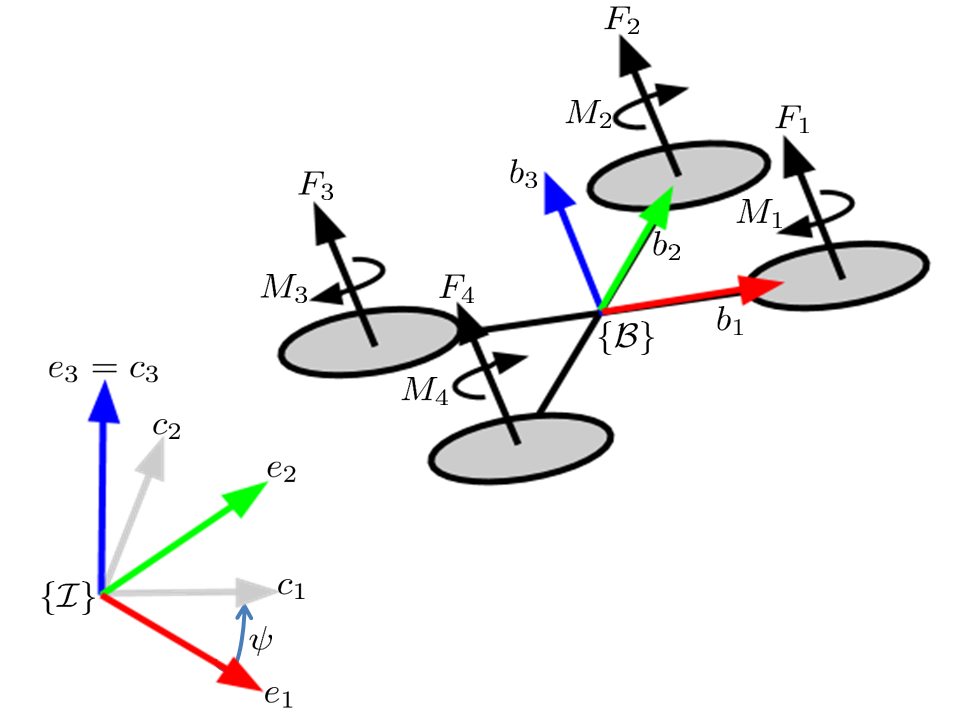
\includegraphics[width=.5\textwidth]{./StyleStuff/qrmodel.png}}}
%%	\makebox[.34\textwidth][c]{\subfloat[][load angles  \label{fig:app.angles}]{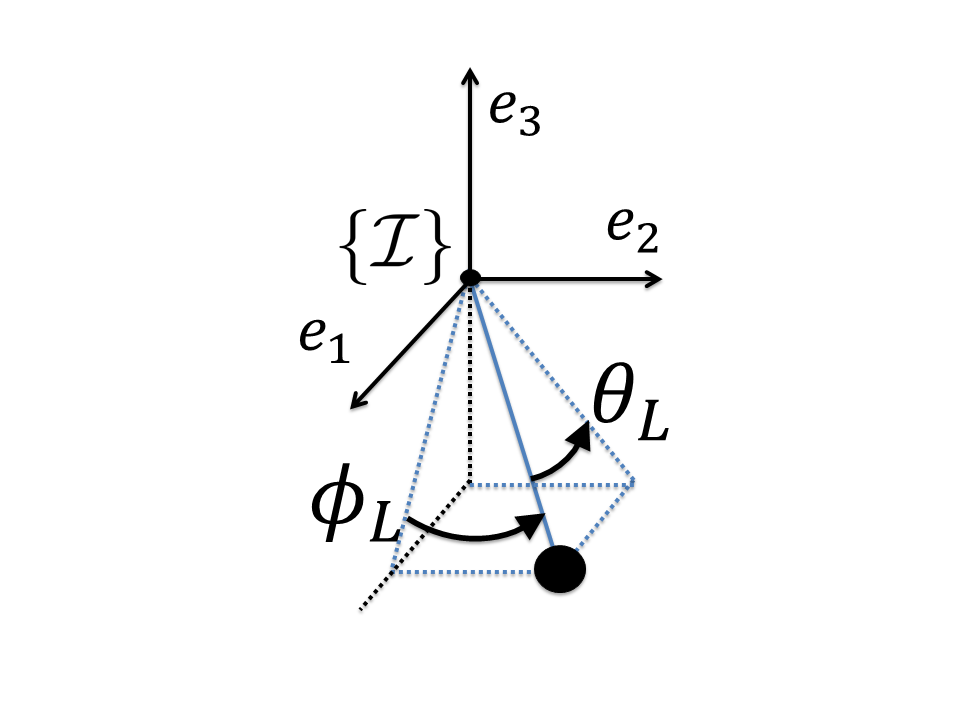
\includegraphics[width=.5\textwidth]{./StyleStuff/angles.png}}}
%%	\caption{Model representation\label{fig:}}
%%\end{figure}		
%
%The following equations of motion follow from Newton's law.
%\begin{equation}\label{eq:newton}
%\begin{aligned}
%\dot{x}_Q &= v_Q\\
%m_Q\dot{v}_Q &=fRe_3-m_Qge_3-Tq\\
%\dot{x}_L &= v_L\\
%m_L\dot{v}_L &=-m_Lge_3+Tq
%\end{aligned}
%\end{equation}
%where $ x_Q = x_L-Lq $. $ T $ is the cable tension, defined by $ T=|f| q $, where $ |f| = m_L\dot{v}_L $ is the magnitude of the force.
%%which gives the following equation, derived in Section \ref{sec.app:loaddyn},
%%\begin{equation}\label{key}
%%%CHECK whether equation is correct
%%(m_Q+m_L)(\dot{v}_L+ge_3)=fRe_3-m_QL\ddot{q}
%%\end{equation}
%
%Because Euler-Angles are used, a function is required that maps a vector of the Z-X-Y Euler angles to its rotation matrix $ R\in SO(3) $, which is denoted as \cite{Mahony2012}
%\begin{equation}\label{key}
%%R_{ZXY}({\phi},{\theta},{\psi})=\begin{bmatrix}
%c_{\psi}c_{\theta}-s_{\phi}s_{\psi}s_{\theta}&-c_{\phi}s_{\psi}&c_{\psi}s_{\theta}+c_{\theta}s_{\phi}s_{\psi}\\
%c_{\theta}s_{\psi}+c_{\psi}s_{\phi}s_{\theta}&c_{\phi}c_{\psi}&s_{\psi}s_{\theta}-c_{\psi}c_{\theta}s_{\phi}\\
%-c_{\phi}s_{\theta}&s_{\phi}&c_{\phi}c_{\theta}
%\end{bmatrix}
%\end{equation}
%The Z-X-Y Euler angles rotate \BF, as can be seen in Figure \ref{fig:app.model}. The first rotation by yaw angle $ \psi $ is around the z-axis of \IF. Next is the rotation by roll angle $ \phi $, and the last rotation is by pitch angle $ \theta $.
%%\begin{figure}[h!]
%%	\centering
%%	\makebox[\textwidth][c]{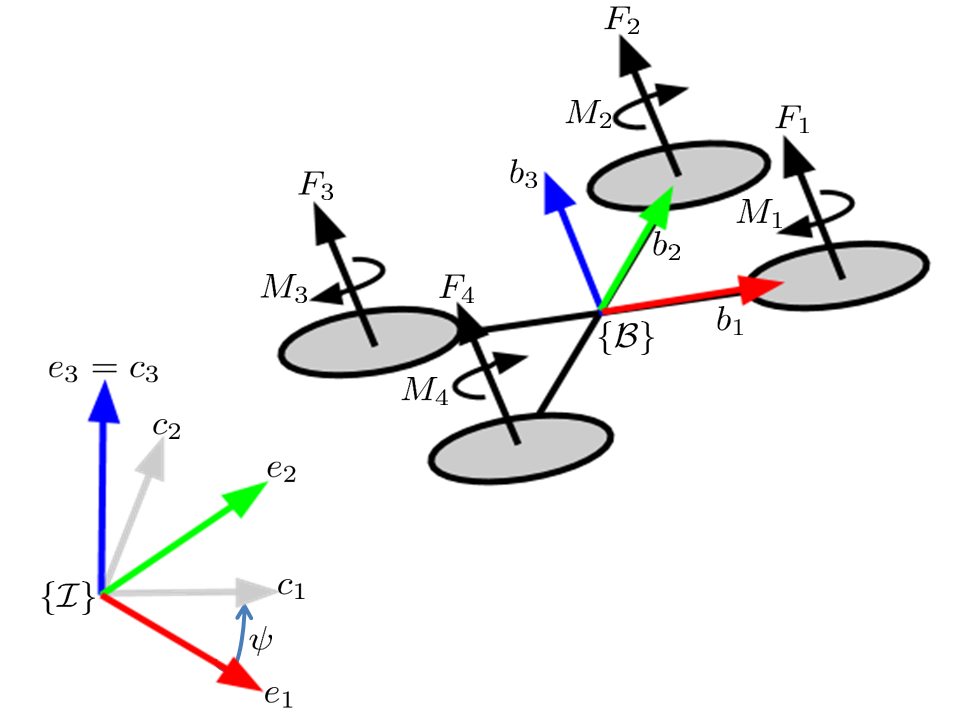
\includegraphics[width=.45\textwidth]{./StyleStuff/qrmodel.png}}
%%	\caption{quadrotor-load model representation\label{fig:mod.modelQRtrad}}
%%\end{figure}
%
%The unit vector $ q $ from the \a{qr} to the load is represented in \BF. Define $ \phi_L $ as the rotation of the load around the z-axis, measured from $ \vec{b}_1 $, and $ \theta_L $ is the angle between the cable and the z-axis of \BF, see Figure \ref{fig:app.angles}.
%The Cartesian coordinates can be retrieved through
%\begin{equation}\label{eq:app.xL2xQ}
%x_L = x_Q+qL
%\end{equation}
%where
%\begin{equation}\label{eq:app.q}
%q=
%\begin{bmatrix}
%s_{\theta_L}c_{\phi_L}\\
%s_{\theta_L}s_{\phi_L}\\
%-c_{\theta_L}
%\end{bmatrix}
%\end{equation}
%\begin{figure}[h!]
%	\centering
%	\makebox[\textwidth][c]{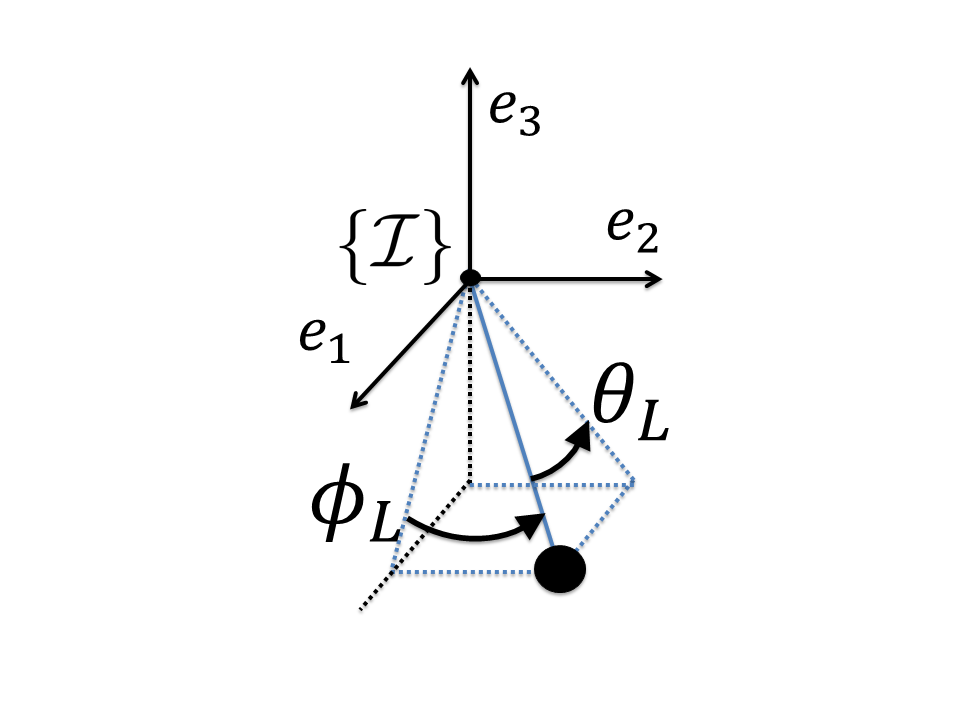
\includegraphics[width=.45\textwidth]{./StyleStuff/angles.png}}
%	\caption{Load angles \label{fig:app.angles}}
%\end{figure}	

%\begin{figure}[h!]
%	\centering
%	\makebox[\textwidth][c]{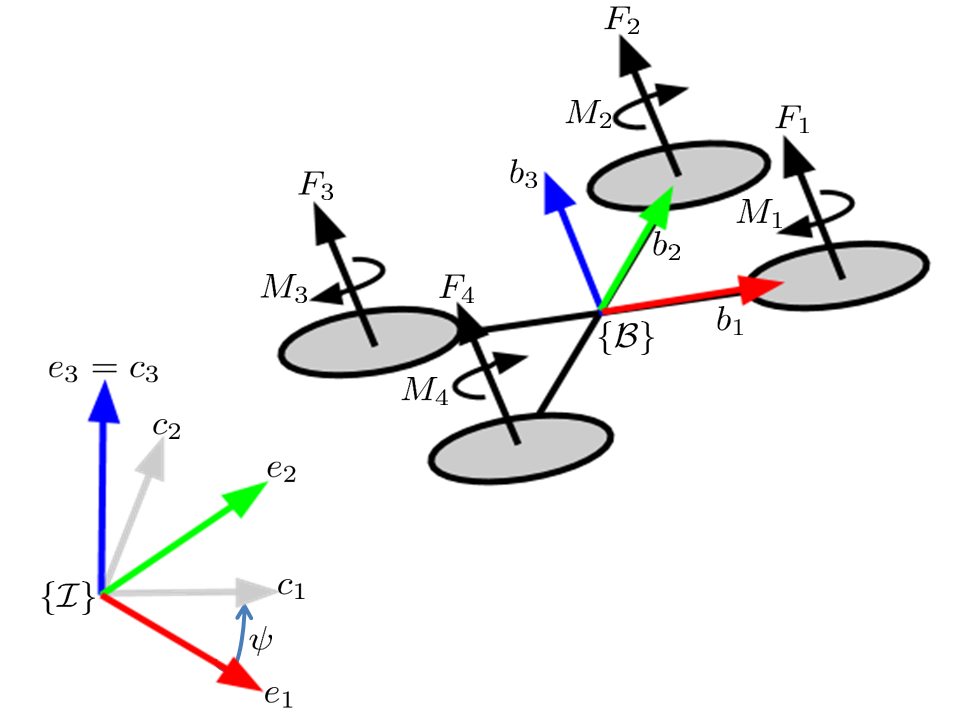
\includegraphics[width=.5\paperwidth]{./StyleStuff/qrmodel.png}}
%	\caption{quadrotor model representation\label{fig:mod.model}}
%\end{figure}	



%\begin{equation}\label{eq:q}
%		q=-R_{\psi_L}R_{\theta_L}e_3=\begin{bmatrix}
%		s_{\theta_L}c_{\psi_L}\\s_{\theta_L}s_{\psi_L}\\-c_{\theta_L}
%		\end{bmatrix}
%\begin{align}
%q=\begin{bmatrix}
%s_{\theta_L}c_{\phi_L}\\
%s_{\theta_L}s_{\phi_L}\\
%c_{\theta_L}
%\end{bmatrix}
%\dot{q}&=\begin{bmatrix}
%s_{\theta_L}c_{\psi_L}\\
%s_{\theta_L}s_{\psi_L}\\
%c_{\theta_L}
%\end{bmatrix}\\
%\end{align}
%\end{equation}  
%Differentiating Equation \ref{eq:app.xL2xQ} and \ref{eq:app.q} gives
%\begin{equation}\label{key}
%\begin{aligned}
%\ddot{x}_L&=\ddot{x}_Q+\ddot{q}L\\
%\ddot{q}&=\begin{bmatrix}
%\ddot{\theta}_Lc_{\theta_L}c_{\phi_L}-\ddot{\phi}_Ls_{\theta_L}s_{\phi_L}-\dot{\phi}_L^2s_{\theta_L}c_{\phi_L}-\dot{\theta}_L^2s_{\theta_L}c_{\phi_L}-2\dot{\theta}_L\dot{\phi}_Lc_{\theta_L}s_{\phi_L}\\
%\ddot{\theta}_Lc_{\theta_L}s_{\phi_L}+\ddot{\phi}_Ls_{\theta_L}c_{\phi_L}-\dot{\phi}_L^2s_{\theta_L}s_{\phi_L}-\dot{\theta}_L^2s_{\theta_L}s_{\phi_L}+2\dot{\theta}_L\dot{\phi}_Lc_{\theta_L}c_{\phi_L}\\
%\ddot{\theta}_Ls_{\theta_L}+\dot{\theta}_L^2 c_{\theta_L}\\
%\end{bmatrix}
%\end{aligned}
%\end{equation}
%
%\begin{equation}\label{key}
%\begin{aligned}
%\ddot{x}_Q&=\frac{1}{m_Q}(f(c_{\psi}s_{\theta}+c_{\theta}s_{\phi}s_{\psi})-Ts_{\theta_L}c_{\psi_L})\\
%\ddot{y}_Q&=\frac{1}{m_Q}(f(s_{\psi}s_{\theta}-c_{\psi}c_{\theta}s_{\phi})-Ts_{\theta_L}s_{\psi_L})\\
%\ddot{z}_Q&=\frac{1}{m_Q}(f(c_{\phi}c_{\theta})-Tc_{\theta_L})-g\\
%\end{aligned}
%\end{equation}

%\begin{align}\label{key}
%%CHECK wat is hier de bedoeling van? Checken in Garcia of literatuur?
%\ddot{\psi}&=\tilde{\tau}_{\psi}\\
%\ddot{\theta}&=\tilde{\tau}_{\theta}\\
%\ddot{\phi} &=\tilde{\tau}_{\phi}
%\end{align}

%
%\section{Figures}
%%CHECK nodig?
%\begin{figure}[h!]
%	\centering
%	\makebox[\textwidth][c]{\includegraphics[width=.45\textwidth]{./StyleStuff/dcsc.png}}
%	\caption{Simulink Command Filter\label{fig:app.CF}}
%\end{figure}		

%\section{\texttt{MATLAB} code}
%\subsection{A \matlab Listing}
%
%\lstset{language=matlab}
%\lstinputlisting{test.m}

%    \subsection{An appendix subsection with C++ Listing}
%
%    \lstset{language=C++}
%    \lstinputlisting{test.c}    

%    \chapter{Appendix: Figures}
%
%    \section{Test section (again?)}
%
%    Ok, all is well.
\newpage
\section{Additional Figures}
Figures \ref{fig:set.caseAinputs}, \ref{fig:set.caseBinputs}, \ref{fig:set.caseBBinputs} and \ref{fig:set.caseCinputs} show the control inputs corresponding to the experiments in cases A, B, B extended and C, respectively. Left are the total force and forces per rotor, right are the moments about the body axes.
\begin{figure}[h!]
	\centering
	\makebox[.49\textwidth][c]{\subfloat[][]{\includegraphics[width=.49\textwidth]{\dir{LPOSQRL-f\caseA}}\label{fig:Af}}}	
	\makebox[.49\textwidth][c]{\subfloat[][]{\includegraphics[width=.49\textwidth]{\dir{LPOSQRL-M\caseA}}\label{fig:AM}}}
	\caption{Control Inputs \a{ngc} Case A \label{fig:set.caseAinputs}}
\end{figure}
\begin{figure}[h!]
	\centering
	\makebox[.49\textwidth][c]{\subfloat[][]{\includegraphics[width=.49\textwidth]{\dir{LPOSQRL-f\caseB}}\label{fig:Bf}}}	
	\makebox[.49\textwidth][c]{\subfloat[][]{\includegraphics[width=.49\textwidth]{\dir{LPOSQRL-M\caseB}}\label{fig:BM}}}
	\caption{Control Inputs \a{ngc} Case B \label{fig:set.caseBinputs}}
\end{figure}
\begin{figure}[h!]
	\centering
	\makebox[.49\textwidth][c]{\subfloat[][]{\includegraphics[width=.49\textwidth]{\dir{LPOSQRL-f\caseBB}}\label{fig:BBf}}}	
	\makebox[.49\textwidth][c]{\subfloat[][]{\includegraphics[width=.49\textwidth]{\dir{LPOSQRL-M\caseBB}}\label{fig:BBM}}}
	\caption{Control Inputs \a{ngc} Case B extended \label{fig:set.caseBBinputs}}
\end{figure}
\begin{figure}[h!]
	\centering
	\makebox[.49\textwidth][c]{\subfloat[][]{\includegraphics[width=.49\textwidth]{\dir{LPOSQRL-f\caseC}}\label{fig:Cf}}}	
	\makebox[.49\textwidth][c]{\subfloat[][]{\includegraphics[width=.49\textwidth]{\dir{LPOSQRL-M\caseC}}\label{fig:CM}}}
	\caption{Control Inputs \a{ngc} Case C \label{fig:set.caseCinputs}}
\end{figure}
\clearpage

%
%Figures \ref{fig:caseALQRe}, \ref{fig:caseBLQRe}, \ref{fig:caseBBLQRe} and \ref{fig:caseCLQRe} show the \a{qr} position and load angle tracking error corresponding to the experiments done with the \a{lqr} controller in cases A, B, B extended and C, respectively.
%\begin{figure}[h!]
%	\centering
%	\makebox[.49\textwidth][c]{\subfloat[][]{\includegraphics[width=.49\textwidth]{\dir{LQR-exQ\caseA}}\label{fig:}}}	
%	\makebox[.49\textwidth][c]{\subfloat[][]{\includegraphics[width=.49\textwidth]{\dir{LQR-exL\caseA}}\label{fig:}}}
%	\caption{\a{qr} Position Error and Load Angle Error \a{lqr} Case A. Dash-dot: \a{lqr}\label{fig:caseALQRe}}
%\end{figure}		
%\begin{figure}[h!]
%	\centering
%	\makebox[.49\textwidth][c]{\subfloat[][]{\includegraphics[width=.49\textwidth]{\dir{LQR-exQ\caseB}}\label{fig:}}}	
%	\makebox[.49\textwidth][c]{\subfloat[][]{\includegraphics[width=.49\textwidth]{\dir{LQR-exL\caseB}}\label{fig:}}}
%	\caption{\a{qr} Position Error and Load Angle Error \a{lqr} Case B. Dash-dot: \a{lqr}\label{fig:caseBLQRe}}
%\end{figure}		
%\begin{figure}[h!]
%	\centering
%	\makebox[.49\textwidth][c]{\subfloat[][]{\includegraphics[width=.49\textwidth]{\dir{LQR-exQ\caseBB}}\label{fig:}}}	
%	\makebox[.49\textwidth][c]{\subfloat[][]{\includegraphics[width=.49\textwidth]{\dir{LQR-exL\caseBB}}\label{fig:}}}
%	\caption{\a{qr} Position Error and Load Angle Error \a{lqr} Case B extended. Dash-dot: \a{lqr}\label{fig:caseBBLQRe}}
%\end{figure}		
%\begin{figure}[h!]
%	\centering
%	\makebox[.49\textwidth][c]{\subfloat[][]{\includegraphics[width=.49\textwidth]{\dir{LQR-exQ\caseC}}\label{fig:}}}	
%	\makebox[.49\textwidth][c]{\subfloat[][]{\includegraphics[width=.49\textwidth]{\dir{LQR-exL\caseC}}\label{fig:}}}
%	\caption{\a{qr} Position Error and Load Angle Error \a{lqr} Case C. Dash-dot: \a{lqr}\label{fig:caseCLQRe}}
%\end{figure}		


